\documentclass[12pt]{article}
\usepackage{tikz}

\title{CPSC 3400 - Homework 6 \\
DFAs, Regular Expressions and Turing machines}

\author{Minh-Hieu Nguyen}
\date{May 28, 2022}


\begin{document}

\maketitle

\section*{Part I. DFAs}

Draw DFAs for the following language specifications.

\begin{enumerate}
    \item All strings on $\sum = \{A,B,C\}$ that contain each letter ($A$, $B$, and $C$) at least once.

          \begin{center}
              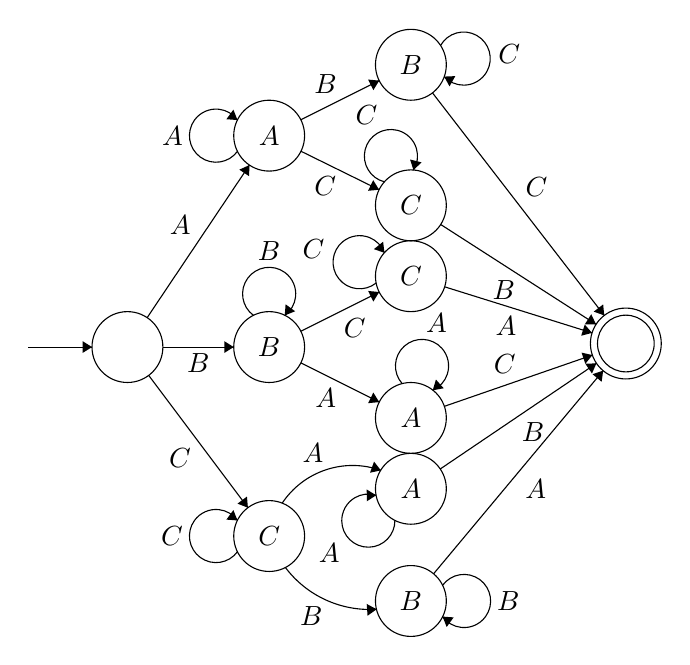
\begin{tikzpicture}[scale=0.15]
                  \tikzstyle{every node}+=[inner sep=0pt]
                  \draw [black] (8.9,-30.1) circle (3);
                  \draw [black] (20.9,-12.2) circle (3);
                  \draw (20.9,-12.2) node {$A$};
                  \draw [black] (20.9,-30.1) circle (3);
                  \draw (20.9,-30.1) node {$B$};
                  \draw [black] (20.9,-46.1) circle (3);
                  \draw (20.9,-46.1) node {$C$};
                  \draw [black] (32.9,-24.1) circle (3);
                  \draw (32.9,-24.1) node {$C$};
                  \draw [black] (32.9,-18.1) circle (3);
                  \draw (32.9,-18.1) node {$C$};
                  \draw [black] (32.9,-36.1) circle (3);
                  \draw (32.9,-36.1) node {$A$};
                  \draw [black] (32.9,-51.6) circle (3);
                  \draw (32.9,-51.6) node {$B$};
                  \draw [black] (32.9,-6.2) circle (3);
                  \draw (32.9,-6.2) node {$B$};
                  \draw [black] (32.9,-42.1) circle (3);
                  \draw (32.9,-42.1) node {$A$};
                  \draw [black] (51.1,-29.8) circle (3);
                  \draw [black] (51.1,-29.8) circle (2.4);
                  \draw [black] (0.5,-30.1) -- (5.9,-30.1);
                  \fill [black] (5.9,-30.1) -- (5.1,-29.6) -- (5.1,-30.6);
                  \draw [black] (11.9,-30.1) -- (17.9,-30.1);
                  \fill [black] (17.9,-30.1) -- (17.1,-29.6) -- (17.1,-30.6);
                  \draw (14.9,-30.6) node [below] {$B$};
                  \draw [black] (10.57,-27.61) -- (19.23,-14.69);
                  \fill [black] (19.23,-14.69) -- (18.37,-15.08) -- (19.2,-15.63);
                  \draw (14.29,-19.81) node [left] {$A$};
                  \draw [black] (10.7,-32.5) -- (19.1,-43.7);
                  \fill [black] (19.1,-43.7) -- (19.02,-42.76) -- (18.22,-43.36);
                  \draw (14.32,-39.5) node [left] {$C$};
                  \draw [black] (23.59,-13.52) -- (30.21,-16.78);
                  \fill [black] (30.21,-16.78) -- (29.71,-15.97) -- (29.27,-16.87);
                  \draw (25.65,-15.66) node [below] {$C$};
                  \draw [black] (23.58,-10.86) -- (30.22,-7.54);
                  \fill [black] (30.22,-7.54) -- (29.28,-7.45) -- (29.72,-8.35);
                  \draw (25.68,-8.69) node [above] {$B$};
                  \draw [black] (23.58,-28.76) -- (30.22,-25.44);
                  \fill [black] (30.22,-25.44) -- (29.28,-25.35) -- (29.72,-26.25);
                  \draw (28.15,-27.61) node [below] {$C$};
                  \draw [black] (23.58,-31.44) -- (30.22,-34.76);
                  \fill [black] (30.22,-34.76) -- (29.72,-33.95) -- (29.28,-34.85);
                  \draw (25.69,-33.61) node [below] {$A$};
                  \draw [black] (21.994,-43.33) arc (146.45435:70.41554:7.162);
                  \fill [black] (30.36,-40.54) -- (29.78,-39.8) -- (29.44,-40.74);
                  \draw (24.61,-39.95) node [above] {$A$};
                  \draw [black] (29.997,-52.297) arc (-86.14129:-143.10584:8.915);
                  \fill [black] (30,-52.3) -- (29.16,-51.85) -- (29.23,-52.85);
                  \draw (24.47,-52.02) node [below] {$B$};
                  \draw [black] (34.73,-8.58) -- (49.27,-27.42);
                  \fill [black] (49.27,-27.42) -- (49.18,-26.49) -- (48.38,-27.1);
                  \draw (42.57,-16.59) node [right] {$C$};
                  \draw [black] (35.42,-19.72) -- (48.58,-28.18);
                  \fill [black] (48.58,-28.18) -- (48.17,-27.32) -- (47.63,-28.17);
                  \draw (40.76,-24.45) node [below] {$B$};
                  \draw [black] (35.76,-25) -- (48.24,-28.9);
                  \fill [black] (48.24,-28.9) -- (47.62,-28.19) -- (47.32,-29.14);
                  \draw (40.95,-27.5) node [below] {$A$};
                  \draw [black] (35.73,-35.12) -- (48.27,-30.78);
                  \fill [black] (48.27,-30.78) -- (47.35,-30.57) -- (47.67,-31.52);
                  \draw (40.85,-32.41) node [above] {$C$};
                  \draw [black] (35.39,-40.42) -- (48.61,-31.48);
                  \fill [black] (48.61,-31.48) -- (47.67,-31.51) -- (48.23,-32.34);
                  \draw (43.24,-36.45) node [below] {$B$};
                  \draw [black] (34.82,-49.3) -- (49.18,-32.1);
                  \fill [black] (49.18,-32.1) -- (48.28,-32.4) -- (49.05,-33.04);
                  \draw (42.55,-42.14) node [right] {$A$};
                  \draw [black] (18.22,-13.523) arc (-36:-324:2.25);
                  \draw (13.65,-12.2) node [left] {$A$};
                  \fill [black] (18.22,-10.88) -- (17.87,-10) -- (17.28,-10.81);
                  \draw [black] (35.407,-4.574) arc (150.70469:-137.29531:2.25);
                  \draw (40.27,-5.29) node [right] {$C$};
                  \fill [black] (35.72,-7.2) -- (36.17,-8.03) -- (36.66,-7.16);
                  \draw [black] (30.668,-16.113) arc (256.05831:-31.94169:2.25);
                  \draw (29.15,-11.32) node [above] {$C$};
                  \fill [black] (33.12,-15.12) -- (33.8,-14.46) -- (32.83,-14.22);
                  \draw [black] (29.967,-24.671) arc (308.74488:20.74488:2.25);
                  \draw (25.62,-21.8) node [left] {$C$};
                  \fill [black] (30.66,-22.12) -- (30.55,-21.18) -- (29.77,-21.81);
                  \draw [black] (32.168,-33.203) arc (221.90524:-66.09476:2.25);
                  \draw (35.06,-28.9) node [above] {$A$};
                  \fill [black] (34.75,-33.76) -- (35.68,-33.59) -- (35.02,-32.85);
                  \draw [black] (31.546,-44.764) arc (0.79457:-287.20543:2.25);
                  \draw (26.92,-47.54) node [left] {$A$};
                  \fill [black] (29.96,-42.65) -- (29.16,-42.16) -- (29.17,-43.16);
                  \draw [black] (35.58,-50.277) arc (144:-144:2.25);
                  \draw (40.15,-51.6) node [right] {$B$};
                  \fill [black] (35.58,-52.92) -- (35.93,-53.8) -- (36.52,-52.99);
                  \draw [black] (18.22,-47.423) arc (324:36:2.25);
                  \draw (13.65,-46.1) node [left] {$C$};
                  \fill [black] (18.22,-44.78) -- (17.87,-43.9) -- (17.28,-44.71);
                  \draw [black] (19.577,-27.42) arc (234:-54:2.25);
                  \draw (20.9,-22.85) node [above] {$B$};
                  \fill [black] (22.22,-27.42) -- (23.1,-27.07) -- (22.29,-26.48);
              \end{tikzpicture}
          \end{center}

    \item All strings on $\sum = \{X,Y,Z\}$ that contain two secutive $X$s or three consecutive $Z$s (or both).

          \centering{\textbf{Solution}}
          \begin{center}
              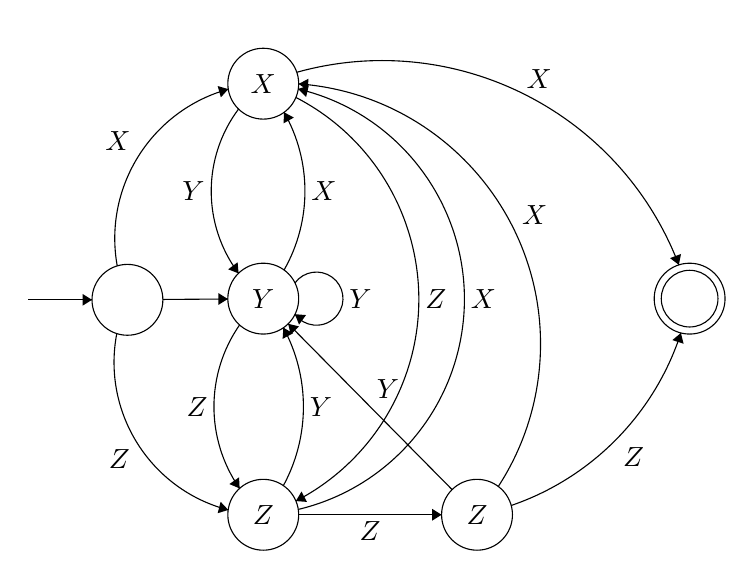
\begin{tikzpicture}[scale=0.15]
                  \tikzstyle{every node}+=[inner sep=0pt]
                  \draw [black] (9.3,-30.1) circle (3);
                  \draw [black] (20.8,-30) circle (3);
                  \draw (20.8,-30) node {$Y$};
                  \draw [black] (20.8,-48.3) circle (3);
                  \draw (20.8,-48.3) node {$Z$};
                  \draw [black] (20.8,-11.8) circle (3);
                  \draw (20.8,-11.8) node {$X$};
                  \draw [black] (38.9,-48.3) circle (3);
                  \draw (38.9,-48.3) node {$Z$};
                  \draw [black] (56.9,-30) circle (3);
                  \draw [black] (56.9,-30) circle (2.4);
                  \draw [black] (0.9,-30.1) -- (6.3,-30.1);
                  \fill [black] (6.3,-30.1) -- (5.5,-29.6) -- (5.5,-30.6);
                  \draw [black] (12.3,-30.07) -- (17.8,-30.03);
                  \fill [black] (17.8,-30.03) -- (17,-29.53) -- (17,-30.53);
                  \draw [black] (22.561,-14.221) arc (29.66651:-29.66651:13.494);
                  \fill [black] (22.56,-14.22) -- (22.52,-15.16) -- (23.39,-14.67);
                  \draw (24.83,-20.9) node [right] {$X$};
                  \draw [black] (18.799,-46.075) arc (-145.13229:-214.86771:12.113);
                  \fill [black] (18.8,-46.07) -- (18.75,-45.13) -- (17.93,-45.7);
                  \draw (16.12,-39.15) node [left] {$Z$};
                  \draw [black] (17.835,-47.889) arc (-104.55016:-190.87487:12.913);
                  \fill [black] (17.84,-47.89) -- (17.19,-47.2) -- (16.94,-48.17);
                  \draw (9.54,-43.59) node [left] {$Z$};
                  \draw [black] (8.436,-27.234) arc (-169.77019:-254.52158:13.116);
                  \fill [black] (17.84,-12.26) -- (16.94,-12) -- (17.21,-12.96);
                  \draw (9.61,-16.63) node [left] {$X$};
                  \draw [black] (23.639,-10.835) arc (105.58324:20.90638:26.895);
                  \fill [black] (55.99,-27.14) -- (56.17,-26.22) -- (55.24,-26.57);
                  \draw (44.17,-12.22) node [above] {$X$};
                  \draw [black] (23.8,-48.3) -- (35.9,-48.3);
                  \fill [black] (35.9,-48.3) -- (35.1,-47.8) -- (35.1,-48.8);
                  \draw (29.85,-48.8) node [below] {$Z$};
                  \draw [black] (56.163,-32.906) arc (-17.98372:-71.06927:22.928);
                  \fill [black] (56.16,-32.91) -- (55.44,-33.51) -- (56.39,-33.82);
                  \draw (51.23,-43.38) node [right] {$Z$};
                  \draw [black] (23.798,-11.816) arc (85.7954:-33.04266:22.098);
                  \fill [black] (23.8,-11.82) -- (24.56,-12.37) -- (24.63,-11.38);
                  \draw (42.67,-22.94) node [right] {$X$};
                  \draw [black] (23.762,-12.251) arc (76.64348:-76.64348:18.294);
                  \fill [black] (23.76,-12.25) -- (24.43,-12.92) -- (24.66,-11.95);
                  \draw (38.33,-30.05) node [right] {$X$};
                  \draw [black] (18.712,-27.858) arc (-143.13976:-216.86024:11.599);
                  \fill [black] (18.71,-27.86) -- (18.63,-26.92) -- (17.83,-27.52);
                  \draw (15.89,-20.9) node [left] {$Y$};
                  \draw [black] (22.502,-32.463) arc (28.5082:-28.5082:14.01);
                  \fill [black] (22.5,-32.46) -- (22.44,-33.41) -- (23.32,-32.93);
                  \draw (24.7,-39.15) node [right] {$Y$};
                  \draw [black] (23.562,-12.963) arc (62.69242:-62.69242:19.23);
                  \fill [black] (23.56,-47.14) -- (24.5,-47.21) -- (24.04,-46.33);
                  \draw (34.47,-30.05) node [right] {$Z$};
                  \draw [black] (36.79,-46.17) -- (22.91,-32.13);
                  \fill [black] (22.91,-32.13) -- (23.12,-33.05) -- (23.83,-32.35);
                  \draw (30.37,-37.68) node [right] {$Y$};
                  \draw [black] (23.48,-28.677) arc (144:-144:2.25);
                  \draw (28.05,-30) node [right] {$Y$};
                  \fill [black] (23.48,-31.32) -- (23.83,-32.2) -- (24.42,-31.39);
              \end{tikzpicture}
          \end{center}

    \item All strings on $\sum = \{A,B,C,D\}$ that match the Python regular expression \texttt{\^}\texttt{(A?(B|CD)*A+D)\$}

          \centering{\textbf{Solution}}

          \begin{center}
              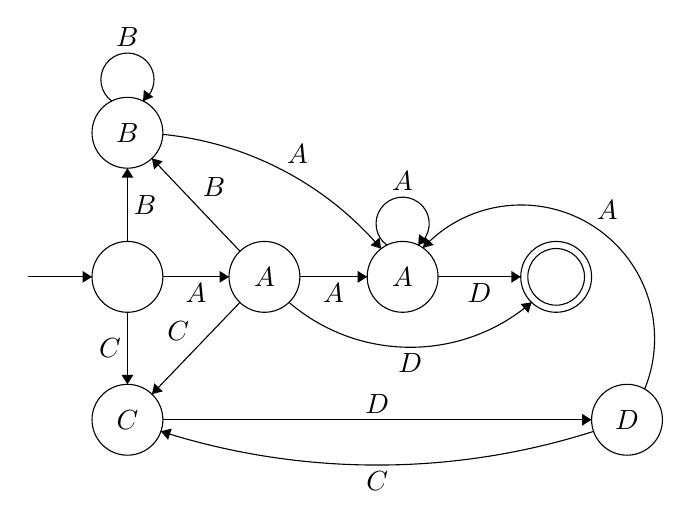
\begin{tikzpicture}[scale=0.15]
                  \tikzstyle{every node}+=[inner sep=0pt]
                  \draw [black] (8.9,-30.1) circle (3);
                  \draw [black] (32.2,-30.1) circle (3);
                  \draw (32.2,-30.1) node {$A$};
                  \draw [black] (45.2,-30.1) circle (3);
                  \draw [black] (45.2,-30.1) circle (2.4);
                  \draw [black] (20.5,-30.1) circle (3);
                  \draw (20.5,-30.1) node {$A$};
                  \draw [black] (8.9,-17.9) circle (3);
                  \draw (8.9,-17.9) node {$B$};
                  \draw [black] (8.9,-42.2) circle (3);
                  \draw (8.9,-42.2) node {$C$};
                  \draw [black] (51.2,-42.2) circle (3);
                  \draw (51.2,-42.2) node {$D$};
                  \draw [black] (0.5,-30.1) -- (5.9,-30.1);
                  \fill [black] (5.9,-30.1) -- (5.1,-29.6) -- (5.1,-30.6);
                  \draw [black] (35.2,-30.1) -- (42.2,-30.1);
                  \fill [black] (42.2,-30.1) -- (41.4,-29.6) -- (41.4,-30.6);
                  \draw (38.7,-30.6) node [below] {$D$};
                  \draw [black] (30.877,-27.42) arc (234:-54:2.25);
                  \draw (32.2,-22.85) node [above] {$A$};
                  \fill [black] (33.52,-27.42) -- (34.4,-27.07) -- (33.59,-26.48);
                  \draw [black] (11.9,-30.1) -- (17.5,-30.1);
                  \fill [black] (17.5,-30.1) -- (16.7,-29.6) -- (16.7,-30.6);
                  \draw (14.7,-30.6) node [below] {$A$};
                  \draw [black] (23.5,-30.1) -- (29.2,-30.1);
                  \fill [black] (29.2,-30.1) -- (28.4,-29.6) -- (28.4,-30.6);
                  \draw (26.35,-30.6) node [below] {$A$};
                  \draw [black] (43.123,-32.258) arc (-49.34933:-130.65067:15.769);
                  \fill [black] (43.12,-32.26) -- (42.19,-32.4) -- (42.84,-33.16);
                  \draw (32.85,-36.56) node [below] {$D$};
                  \draw [black] (8.9,-27.1) -- (8.9,-20.9);
                  \fill [black] (8.9,-20.9) -- (8.4,-21.7) -- (9.4,-21.7);
                  \draw (9.4,-24) node [right] {$B$};
                  \draw [black] (18.43,-27.93) -- (10.97,-20.07);
                  \fill [black] (10.97,-20.07) -- (11.16,-21) -- (11.88,-20.31);
                  \draw (15.23,-22.53) node [right] {$B$};
                  \draw [black] (11.895,-18.036) arc (84.32293:40.40349:27.901);
                  \fill [black] (30.38,-27.72) -- (30.24,-26.78) -- (29.48,-27.43);
                  \draw (23.29,-20.58) node [above] {$A$};
                  \draw [black] (7.577,-15.22) arc (234:-54:2.25);
                  \draw (8.9,-10.65) node [above] {$B$};
                  \fill [black] (10.22,-15.22) -- (11.1,-14.87) -- (10.29,-14.28);
                  \draw [black] (8.9,-33.1) -- (8.9,-39.2);
                  \fill [black] (8.9,-39.2) -- (9.4,-38.4) -- (8.4,-38.4);
                  \draw (8.4,-36.15) node [left] {$C$};
                  \draw [black] (11.9,-42.2) -- (48.2,-42.2);
                  \fill [black] (48.2,-42.2) -- (47.4,-41.7) -- (47.4,-42.7);
                  \draw (30.05,-41.7) node [above] {$D$};
                  \draw [black] (48.366,-43.183) arc (-72.29431:-107.70569:60.225);
                  \fill [black] (11.73,-43.18) -- (12.34,-43.9) -- (12.65,-42.95);
                  \draw (30.05,-46.54) node [below] {$C$};
                  \draw [black] (18.42,-32.27) -- (10.98,-40.03);
                  \fill [black] (10.98,-40.03) -- (11.89,-39.8) -- (11.17,-39.11);
                  \draw (14.17,-34.68) node [left] {$C$};
                  \draw [black] (33.92,-27.653) arc (137.30189:-22.28329:11.306);
                  \fill [black] (33.92,-27.65) -- (34.83,-27.4) -- (34.09,-26.73);
                  \draw (49.52,-25.28) node [above] {$A$};
              \end{tikzpicture}
          \end{center}

\end{enumerate}

\section*{Part II. Regular Expressions}

For each item, write a \textbf{\textit{single}} regular expression that mathces that item. Note that in ALL cases, the entire string must match without additional characters.

\begin{enumerate}
    \item A string of digits that contains only digits and contains exactly two fives. Examples of acceptable strings include: "15445", "55", "05563"

          The string should be rejected if it contains anything other than a digits.

          \centerline{\textbf{Solution}}

          \begin{itemize}
              \item Answer: \texttt{\^}\texttt{([0-4,6-9])*(5)([0-4,6-9])*(5)([0-4,6-9])*\$}
              \item Explanation:

                    \begin{itemize}
                        \item \texttt{([0,4,6-9])*}: Accept all strings that contain digits in range from 0 to 9 except 5. It also accept empty strings. (1)
                        \item \texttt{(5)}: Accept only a digit-5 string. (2)
                    \end{itemize}
          \end{itemize}

    \item A regular expression that matches a time expressed in the form "1:45 PM".

          The hours part must be a number from 1 to 12, the minutes range from 00 to 59, and the time must indicate either AM or PM (uppercase only and preceded by exactly one space).

          \centerline{\textbf{Solution}}

          \begin{itemize}
              \item Answer: \texttt{\^}\texttt{((1[0-2]|[1-9]))(:)([0-5][0-9]) ([AP]M)\$}
              \item Explanation:

                    \begin{itemize}
                        \item \texttt{(1[0-2]|[1-9])}: Accept all digit strings that are either in range from 10 to 12 or in range from 0 to 9 without leading zeroes.
                        \item \texttt{(:)}: Accept the separator, "\texttt{:}", between hours and minutes.
                        \item \texttt{([0-5][0-9])}: Accept all digit strings from 00 to 59 (with leading zeroes).
                        \item \texttt{([AP]M)}: Accept "AM" or "PM" with one preceding space to indicate the time meridiem.
                    \end{itemize}
          \end{itemize}

    \item A regular expression that matches a string representing a comma separated list of variable names such as: \texttt{hello, get\_max, sum3}

          \begin{itemize}
              \item A variable name consists of letters, digits, and underscores but cannot start with a digit.
              \item There is exactly one space after every comma. No other spaces are allowed.
              \item Commas and spaces are not allowed before the first name and after the last name.
              \item An empty string is considered a match.
          \end{itemize}

          \centerline{\textbf{Solution}}

          \begin{itemize}
              \item Answer: \texttt{\^}\texttt{\$|}\texttt{\^}\texttt{(([a-zA-Z\_]\textbackslash w*)(, ))*([a-zA-Z\_]\textbackslash w*)\$}
              \item Explanation:

                    \begin{itemize}
                        \item \texttt{\^}\texttt{\$}: Accept empty string.
                        \item \texttt{([a-zA-Z\_]\textbackslash w*)}: Accept variable names that match with the requirements. \texttt{\textbackslash w} is equivalent to \texttt{[a-zA-Z0-9\_]}.
                        \item \texttt{(([a-zA-Z\_]\textbackslash w*)(, ))*}: As the previous one, but addtionally accept previous variable names followed by exactly one comma and one space, if there are more than one variable name.
                    \end{itemize}
          \end{itemize}

\end{enumerate}

\newpage

\section*{Part III. Turing Machines}

Design a Turing machine on the input alphabet \texttt{\{x,y,z\}} that removes all \texttt{z} characters from the input such there are no gaps. If the input string is \texttt{xzzyxzy}, the output should be \texttt{xyxy}.

\begin{itemize}
    \item Hint: The final string does not need to reside on the same part of the tape where it started.
\end{itemize}

\centerline{\textbf{Solution}}


\begin{center}
    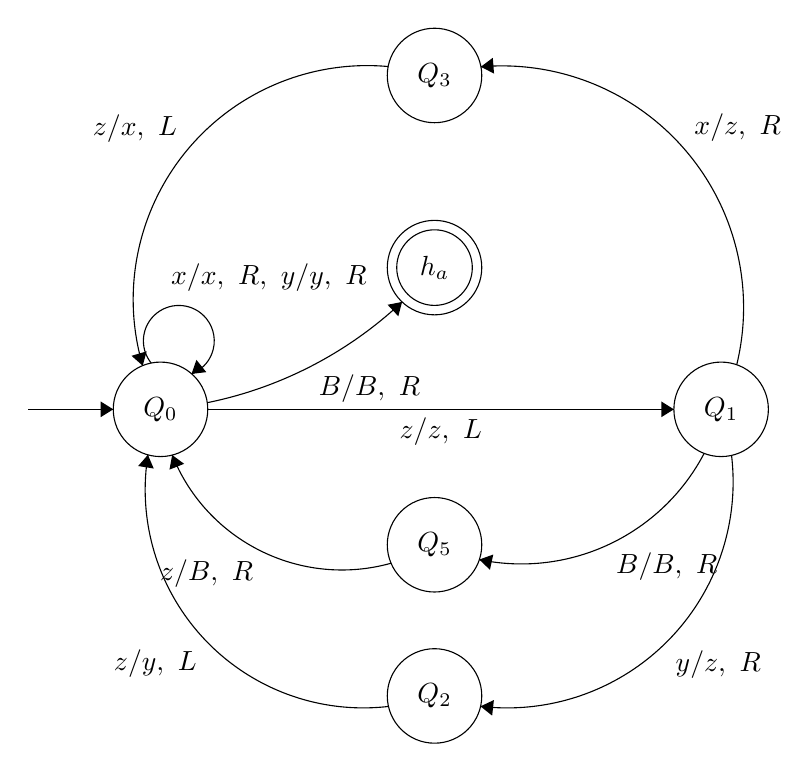
\begin{tikzpicture}[scale=0.2]
        \tikzstyle{every node}+=[inner sep=0pt]
        \draw [black] (8.9,-30.1) circle (3);
        \draw (8.9,-30.1) node {$Q_0$};
        \draw [black] (44.5,-30.1) circle (3);
        \draw (44.5,-30.1) node {$Q_1$};
        \draw [black] (26.3,-48.3) circle (3);
        \draw (26.3,-48.3) node {$Q_2$};
        \draw [black] (26.3,-8.9) circle (3);
        \draw (26.3,-8.9) node {$Q_3$};
        \draw [black] (26.3,-38.7) circle (3);
        \draw (26.3,-38.7) node {$Q_5$};
        \draw [black] (26.3,-21.1) circle (3);
        \draw (26.3,-21.1) node {$h_a$};
        \draw [black] (26.3,-21.1) circle (2.4);
        \draw [black] (0.5,-30.1) -- (5.9,-30.1);
        \fill [black] (5.9,-30.1) -- (5.1,-29.6) -- (5.1,-30.6);
        \draw [black] (8.315,-27.17) arc (219.02894:-68.97106:2.25);
        \draw (15.78,-22.66) node [above] {$x/x,\mbox{ }R,\mbox{ }y/y,\mbox{ }R$};
        \fill [black] (10.87,-27.85) -- (11.81,-27.74) -- (11.18,-26.96);
        \draw [black] (11.9,-30.1) -- (41.5,-30.1);
        \fill [black] (41.5,-30.1) -- (40.7,-29.6) -- (40.7,-30.6);
        \draw (26.7,-30.6) node [below] {$z/z,\mbox{ }L$};
        \draw [black] (29.244,-8.349) arc (94.99805:-13.70649:15.346);
        \fill [black] (29.24,-8.35) -- (30.08,-8.78) -- (30,-7.78);
        \draw (42.77,-12.2) node [right] {$x/z,\mbox{ }R$};
        \draw [black] (7.769,-27.327) arc (-163.59485:-275.16035:14.859);
        \fill [black] (7.77,-27.33) -- (8.02,-26.42) -- (7.06,-26.7);
        \draw (9.98,-12.27) node [left] {$z/x,\mbox{ }L$};
        \draw [black] (45.161,-33.021) arc (6.76892:-96.76892:14.349);
        \fill [black] (29.22,-48.96) -- (29.96,-49.55) -- (30.07,-48.56);
        \draw (41.58,-46.34) node [right] {$y/z,\mbox{ }R$};
        \draw [black] (23.381,-48.966) arc (-83.35953:-189.21513:13.854);
        \fill [black] (8.1,-32.99) -- (7.48,-33.7) -- (8.47,-33.86);
        \draw (11.24,-46.25) node [left] {$z/y,\mbox{ }L$};
        \draw [black] (43.423,-32.893) arc (-27.64299:-101.77297:13.104);
        \fill [black] (29.14,-39.64) -- (29.82,-40.29) -- (30.03,-39.32);
        \draw (41.05,-39.19) node [below] {$B/B,\mbox{ }R$};
        \draw [black] (23.547,-39.871) arc (-74.37047:-158.23156:11.606);
        \fill [black] (9.64,-33) -- (9.47,-33.93) -- (10.4,-33.56);
        \draw (11.83,-39.62) node [below] {$z/B,\mbox{ }R$};
        \draw [black] (24.241,-23.279) arc (-46.75604:-78.54421:25.432);
        \fill [black] (24.24,-23.28) -- (23.32,-23.46) -- (24,-24.19);
        \draw (22.17,-27.86) node [below] {$B/B,\mbox{ }R$};
    \end{tikzpicture}
\end{center}


\end{document}
